%%%%%%%%%%%%%%%%%%%%%%%%%%%%%%%%%%%%%%%%%%%%
% Chapitre 1
%%%%%%%%%%%%%%%%%%%%%%%%%%%%%%%%%%%%%%%%%%%%

\chapter{Imagerie par Résonance Magnétique de diffusion} 
\label{Chapter1}

L'\irmd (IRMd) est une technique d'imagerie \textit{non invasive} 
qui permet de caractériser \textit{in vivo} la structure des fibres de la substance blanche du cerveau humain.
Ce premier chapitre porte sur les notions fondamentales relatives à l'\irmd (IRMd).
Après une brève description des principes de la \rmn (RMN) sur laquelle se base l'IRMd,
sont abordées les notions mathématiques associées à l'IRMd.
% Il commence par une brève descriptions des principes de la \rmn (RMN) sur laquelle se base l'IRMd.
% Après la description de ces points physiques, les notions mathématiques associées à l'IRMd sont abordées.
% Elles servent tout au long de la thèse pour les différentes notations et termes employés.
% Plus particulièrement, cette section introduit le modèle mathématique associé à la diffusion : \og le modèle d'ordre 2 \fg
% et le terme de \og tenseur de diffusion \fg. 
% D'autres modèles mathématiques décrivant la diffusion existent: \og le modèle d'ordre 4 \fg ou encore \og les harmoniques shépriques \fg.
% Cependant, ces modèles n'ont pas été utilisés durant la thèse.
Plus particulièrement, cette section introduit le modèle mathématique associé à la diffusion : \og le modèle du tenseur d'ordre 2 \fg
et le terme de \og tenseur de diffusion \fg. 
Il existe d'autres modèles plus complexes comme \og le modèle du tenseur d'ordre 4 \fg~\cite{Basser1994} 
ou encore \og les harmoniques shépriques \fg~\cite{Barmpoutis2009}.
% qui sont détaillés dans les thèses précédentes \cite{Renard_PhD, Grigis_PhD}.
Cependant, dans ce manuscrit, nous nous attacherons qu'au \og modèle du tenseur d'ordre 2 \fg 
avec en perspective l'idée d'adapter, dans de futurs travaux, les méthodes présentées à des modèles d'ordre supérieur.
% Ils sont détaillés dans les thèses précédentes \cite{Renard_PhD, Grigis_PhD}.
La \figref{fig:irm} est une photographie du scanner IRM SIEMENS de 3 Tesla du laboratoire ICube qui a accueilli cette thèse.

% \minitoc
%----------------------------------------------------------------------------------------
\begin{figure}[h]
    \centering
    \includegraphics[width=0.75\textwidth]{Images/irm_3.pdf}
    \caption{\label{fig:irm} Photographie de l'IRM 3 Tesla du laboratoire ICube à Strasbourg.}
\end{figure}

\section{Principe de l'IRM de diffusion}
L'IRM conventionnelle est une technique qui se base sur le principe de la Résonance Magnétique Nucléaire (RMN).
La RMN utilise les concepts de résonance et d'excitation du spin nucléaire d'une particule chargée, 
le noyau d'hydrogène, présente dans de nombreux tissus organiques dont ceux du cerveau humain.
L'IRMd caractérise, plus particulièrement, le mouvement de ces particules dans plusieurs directions de l'espace.
Le noyau d'hydrogène $H^+$ étant une des composantes de la molécule d'eau $H_2O$,
l'IRMd permet donc de caractériser la diffusion des molécules d'eau dans les tissus.


\subsection{Principe de la Résonance Magnétique Nucléaire (RMN)}
Le noyau d'hydrogène a un moment cinétique, ou \textit{spin}, qui correspond à la rotation de la particule autour d'un axe.
À l'état de repos, les axes de rotation des noyaux d'hydrogène ont des orientations différentes 
comme le montre la représentation en \figref{fig:spins}.
Dès lors qu'un champ magnétique $B_0$ est appliqué, ils se réorientent dans l'axe du champ magnétique 
de manière dite \og parallèle \fg (sens identique à celui de $B_0$) ou \og anti-parallèle \fg (sens opposé).
Ce phénomène est illustré par la \figref{fig:spin_b0}.

\begin{figure}[ht]
    \begin{minipage}[c]{0.45\textwidth}
	    \centering
	    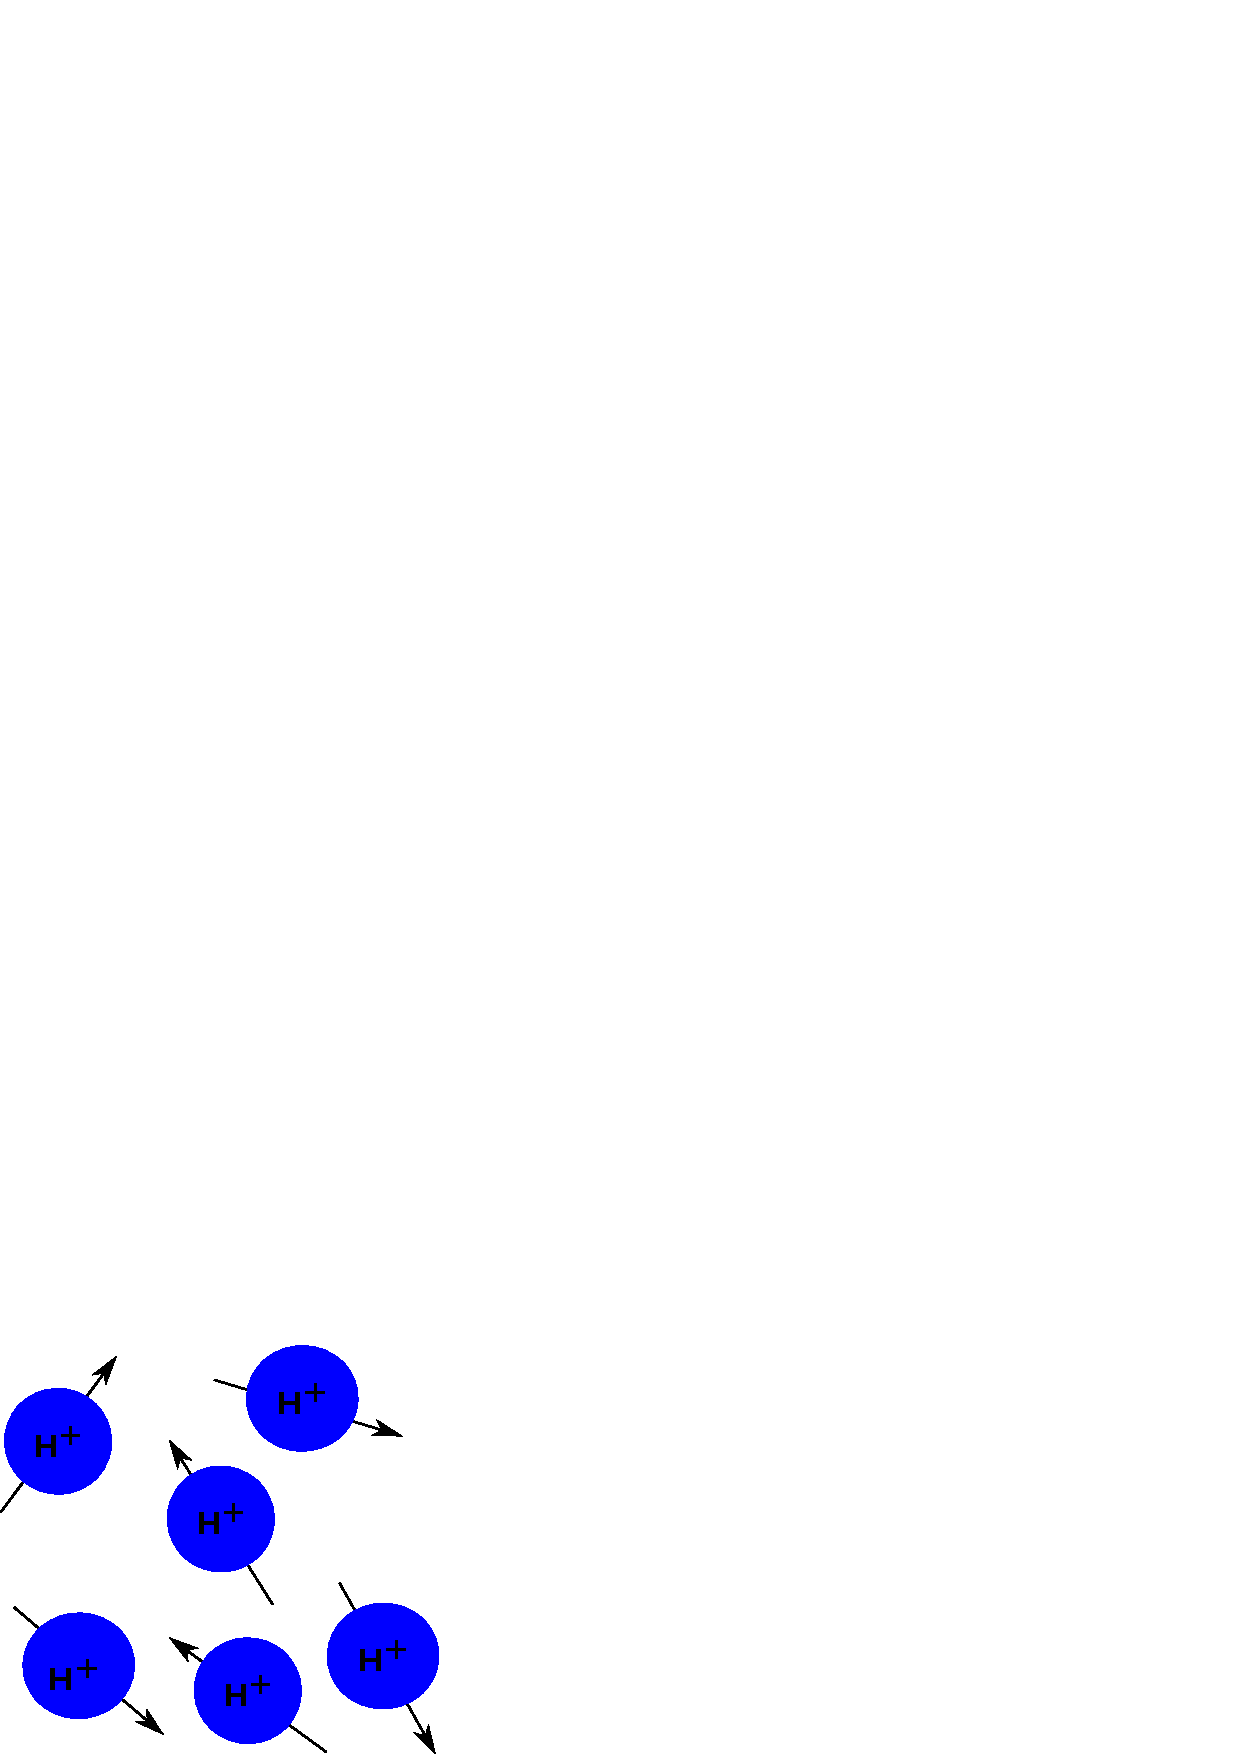
\includegraphics[width=0.75\textwidth]{Images/spins.pdf}
	    \caption{\label{fig:spins}Représentation de noyaux d'hydrogène à l'état de repos.}
    \end{minipage}\hfill
    \begin{minipage}[c]{0.45\textwidth}
	    \centering
	    \includegraphics[width=0.9\textwidth]{Images/spin_b0.pdf}
	    \caption{\label{fig:spin_b0}Représentation de noyaux d'hydrogène dans un champ magnétique $B_0$.}
    \end{minipage}
\end{figure}

Les spins ont alors un mouvement de précession autour de $B_0$ à la fréquence de Larmor $\nu_0$ caractéristique de la particule :
\begin{equation}
    \nu_0 = \frac{\gamma B_0}{2\pi}
\end{equation}
\noindent avec $\gamma=2,675.10^8 \text{ rad}.\text{T}^{-1}.\text{s}^{-1}$ le rapport gyromagnétique propre au noyau d'hydrogène.
Ce mouvement de précession se décompose en deux composantes :
une composante longitudinale suivant l'axe du champ magnétique qui est fixe et une composante transversale qui est en rotation, 
respectivement en jaune et vert sur la \figref{fig:spin_composantes}.

\begin{figure}[ht]
    \begin{minipage}[c]{0.45\textwidth}
	    \centering
	    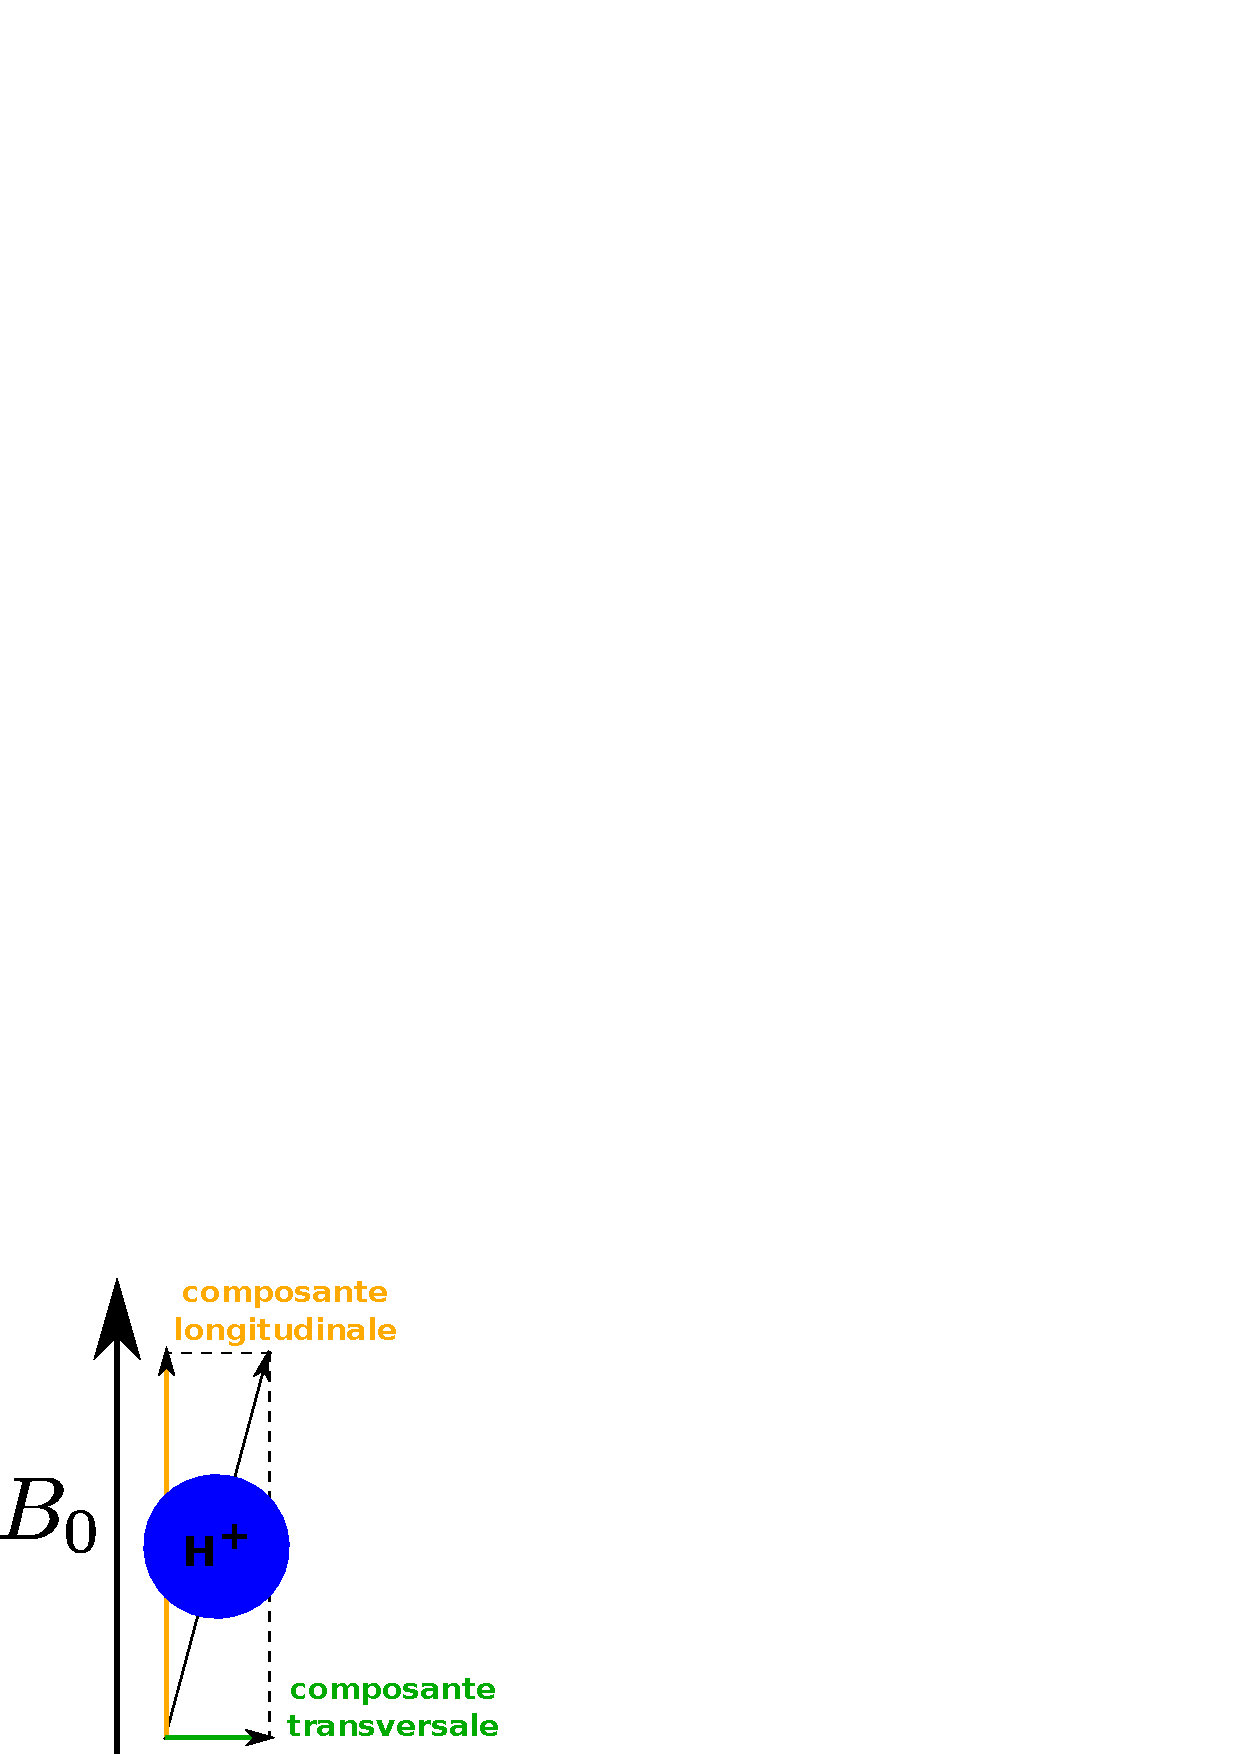
\includegraphics[width=0.7\textwidth]{Images/spin_composantes.pdf}
	    \caption{\label{fig:spin_composantes}Représentation des deux composantes du mouvement de précession d'un noyau d'hydrogène.}
    \end{minipage}\hfill
    \begin{minipage}[c]{0.45\textwidth}
	    \centering
	    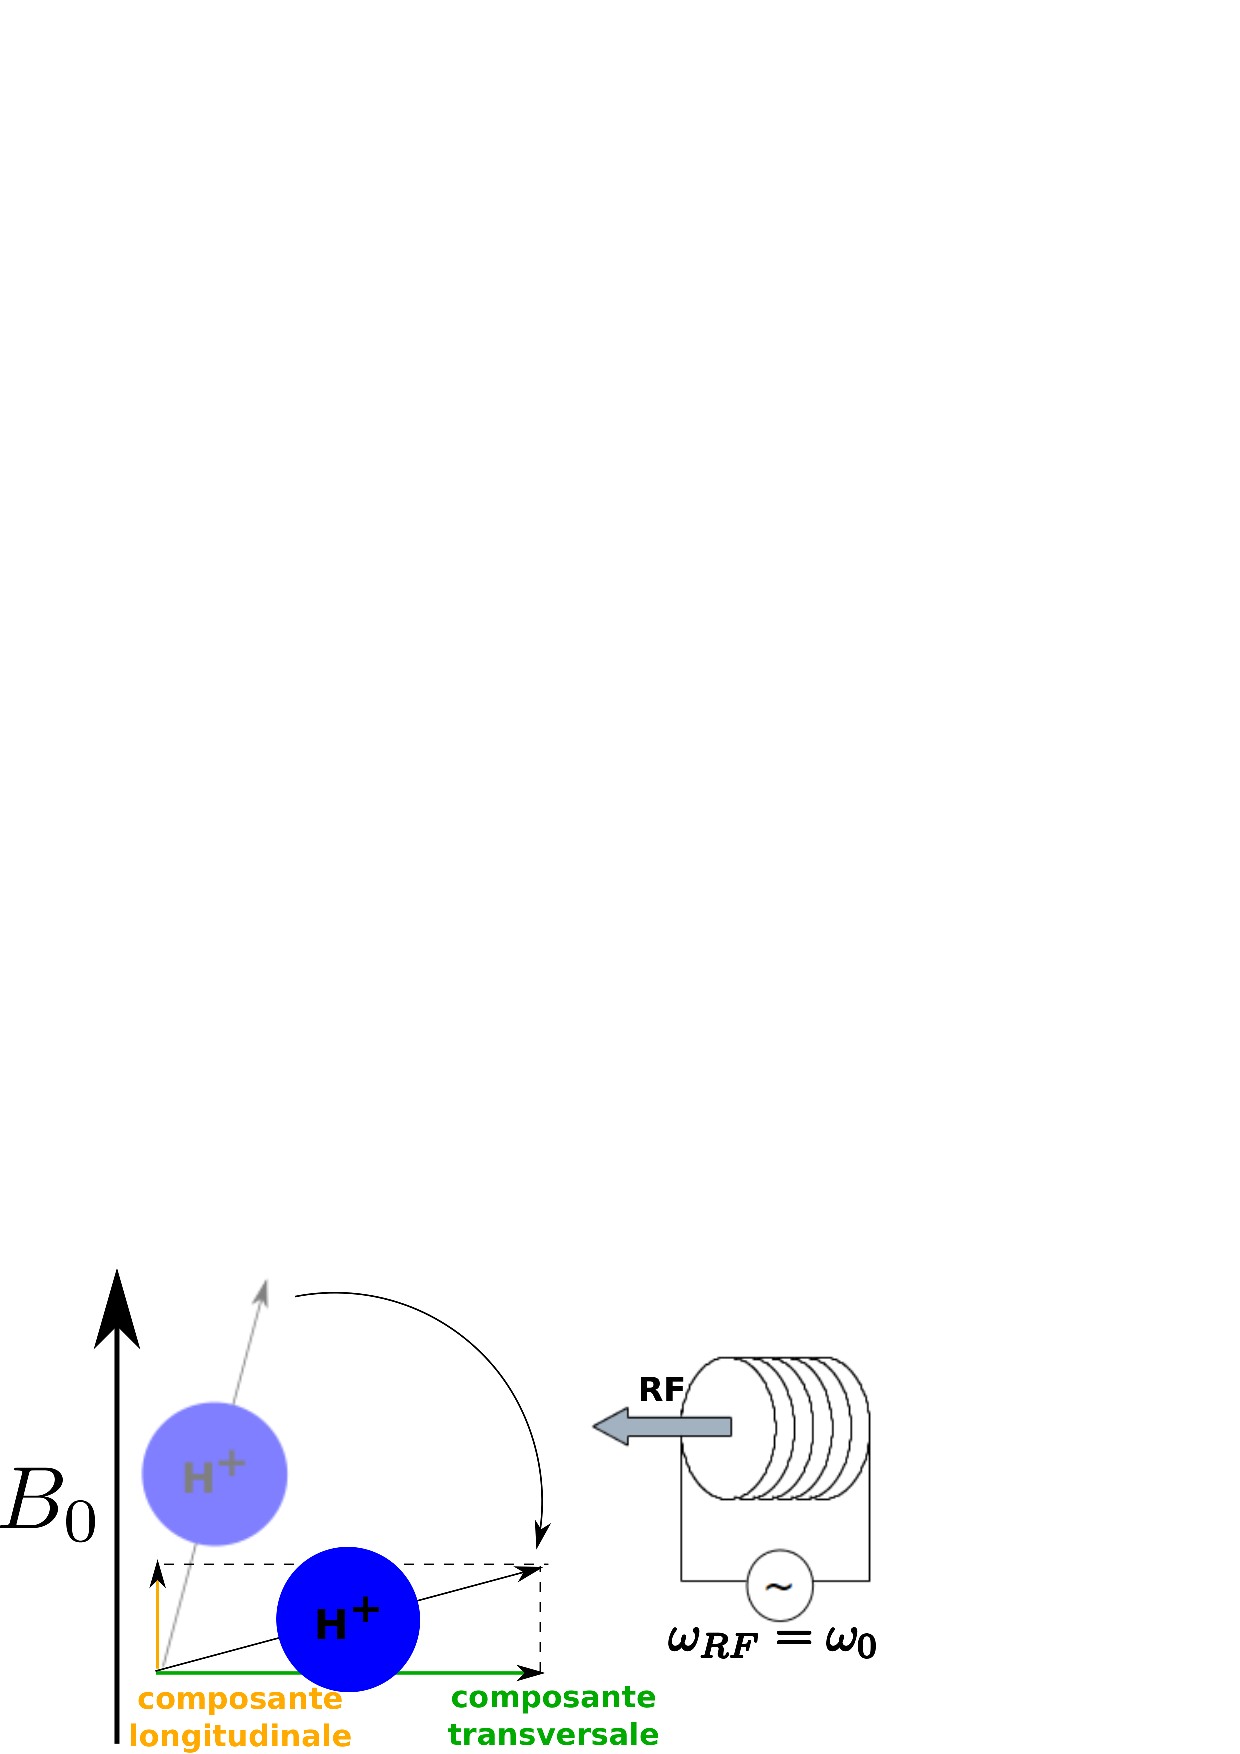
\includegraphics[width=1\textwidth]{Images/excitation.pdf}
	    \caption{\label{fig:excitation}Représentation de la pahse d'excitation.}
    \end{minipage}
\end{figure}

La \rmn consiste à envoyer une onde de Radio-Fréquence (RF) sur ces paticules 
avec une fréquence $\nu_{RF}$ identique à celle de la fréquence de précession $\nu_{0}$.
De cette manière, l'onde RF transmet son énergie aux spins : c'est la phase d'excitation représentée en \figref{fig:excitation}.
Les spins entrent en résonance (\textit{i.e.} ils tournent en phase) et
l'axe de rotation du mouvement de précession bascule.
La composante longitudinale diminue et la composante transversale augmente.
Cette phase d'excitation est suivie par une phase de relaxation durant laquelle les spins retournent à l'état d'équilibre.
Inversement, la composante longitudinale augmente et la composante transversale diminue.
Lors de cette phase, il est possible de mesurer la décroissance de la composante transversale (relaxation $T_2*$)
et avec des séquences particulières, il est possible de mesurer d'autres .

% Lors de cette phase, il est possible de mesurer la décroissance de la composante longitudinale (relaxation $T_1$) 
% ou bien celle de la composante transversale (relaxation $T_2$).
% Lors de cette phase, il est possible de mesurer au cours du temps la composante longitudinale de l'aimantation tissulaire (relaxation $T_1$) 
% ou bien la composante transversale (relaxation $T_2$).

%Ces mesures informent sur l'aimantation globale des tissus.
Pour construire un volume 3D et avoir une valeur par voxel, trois gradients de champ sont utilisés suivant les 3 directions de l'espace. 
Ils servent à la sélection de coupe, au codage en fréquence et au codage en phase.
Les deux derniers gradients définissent la manière dont une matrice $2D$, 
appelée \og espace K \fg, est remplie avec les valeurs de la fréquence spatiale du signal RMN. 
Cette matrice représente ce que nous appelons \og le plan de Fourier \fg et contient les informations pour une seule coupe du volume 3D.
Le module de la transformée de Fourier inverse appliquée à cet espace K permet d'obtenir l'image dans le domaine spatial (signal IRM) 
de la coupe associée (\figref{fig:reconstruction}).
% Une transformée de Fourier inverse est appliquée à cet espace K 
% pour obtenir le signal dans le domaine spatial.
% La magnétude de ce signal permet d'obtenir l'image (signal IRM) de la coupe associée (\figref{fig:reconstruction}).
Le processus est répété pour chaque coupe permettant ainsi de reconstruire le volume 3D.

\begin{figure}[ht]
    \centering
    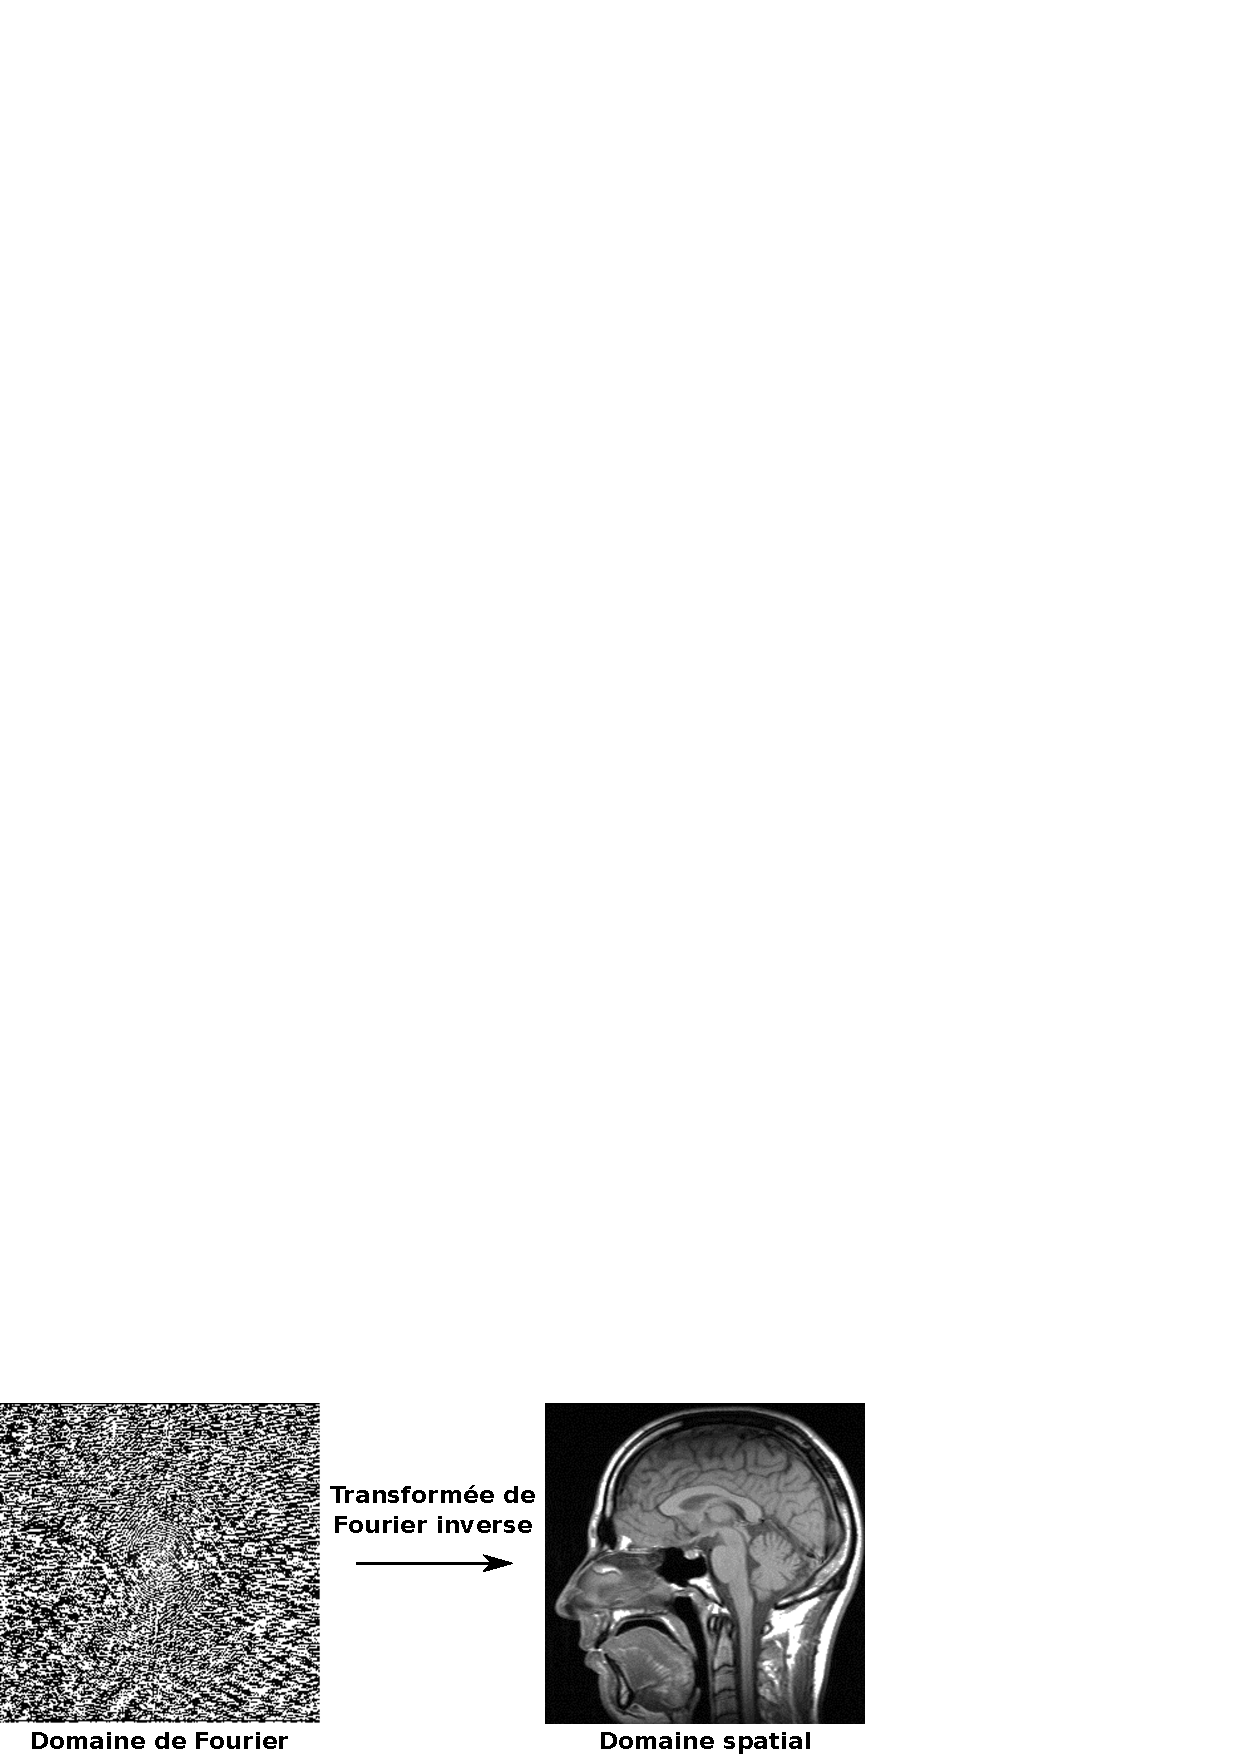
\includegraphics[width=0.8\textwidth]{Images/reconstruction.pdf}
    \caption{\label{fig:reconstruction}Reconstruction d'une coupe 2D à partir du signal acquis dans le domaine de Fourier.}
\end{figure}
Les différentes combinaisons d'ondes RF et de gradients permettent de jouer sur le contraste des tissus, 
la rapidité d'acquisition et l'amélioration du rapport signal sur bruit. 
Cela mène à la création de nouvelles séquences d'acquisition toujours plus performantes.


%\subsection{De la RMN à la diffusion}
%L'\irmd permet de regarder \textit{in vivo} la diffusion des molécules d'eau dans les différents tissus cérébraux.
\subsection{Caractérisation de la diffusion par la RMN}
Ce paragraphe présente la relation entre le principe de la RMN (expliquée précédemment) 
et celui de l'\irmd qui permet de caractériser \textit{in vivo} la diffusion des molécules d'eau dans les différents tissus cérébraux.
Nous commencerons donc par définir le phénomène de diffusion d'une molécule d'eau 
pour aboutir à l'expression liant le signal RMN avec la mesure de la diffusion \eqref{eq:stejskal1965_simple}.\\

Une description rapide du phénomène de diffusion peut être la suivante.
%Le phénomène de diffusion peut être vu de la façon suivante.
Une particule $H^+$ est initialement à la position spatiale $\mathbf{r_0}$.
La probabilité qu'elle se retrouve à la position $\mathbf{r_1}$ après temps $t$ s'écrit $p(\mathbf{r_0}, \mathbf{r_1}, t)$,
souvent notée $p(\mathbf{r}, t)$ avec $\mathbf{r}=\mathbf{r_1} - \mathbf{r_0}$ le vecteur de déplacement.
Cette probabilité, communément appelée \textit{propagateur}, décrit le
déplacement des molécules suivant $I$ directions spatiales $\mathbf{g_{i=0\dots I}}$, 
appelées gradients de diffusion, durant un intervalle de temps $\triangle t$.
Il contient toute l'information relative à la diffusion des molécules d'eau.

En 1965, Stejskal et Tanner \cite{Stejskal1965} mettent en relation le signal acquis par l'IRM $S$
et le propagateur décrivant la diffusion des molécules au cours du temps \eqref{eq:stejskal1965}.
Cette relation montre que le signal $S$ est atténué à cause de l'application des gradients de diffusion : 
les gradients de diffusion déphasent les spins des particules et les rephasent après un durée $\Delta t$ 
au cours de laquelle les particules se sont déplacées spatialement suivant le principe de la diffusion.
À cause de ces déplacements, le rephasage peut ne pas être optimal et cela entraîne un déphasage.
\begin{equation}
    S(\mathbf{g_i},t) = S_0 \int_{voxel} p(\mathbf{r},t)\exp(i\gamma\delta\mathbf{g_i}^T\mathbf{r})d\mathbf{r}
    \label{eq:stejskal1965}
\end{equation}
\noindent avec $S_0$ le signal IRM (acquis sans gradient de diffusion) pondéré en $T_2$, $\gamma$ le rapport gyromagnétique des particules $H^+$ 
et $\delta$ correspondant à la durée d'application du gradient de diffusion.\\

Dans l'équation \eqref{eq:stejskal1965}, l'information de la diffusion est portée par le propagateur $p(\mathbf{r},t)$.
Cependant, c'est une fonction mathématique très complexe attribuant une valeur salaire (probabilité)
depuis un vecteur de déplacements $\mathbf{r}$ et un intervalle de temps $t$ : $p(\mathbf{r},t)\ :\ \mathbb{R}^3\times\mathbb{R} \mapsto \mathbb{R}$.
Cette complexité rend l'analyse de la diffusion difficile.
Dans l'optique de simplifier l'équation \eqref{eq:stejskal1965}, le propagateur peut être modélisé par des outils mathématiques plus simples
tels que le tenseur de diffusion d'ordre 2~\cite{Basser1994} ou d'ordre 4~\cite{Barmpoutis2009} ou les harmoniques sphériques~\cite{Descoteaux2007}.
Dans la littérature, le modèle d'ordre 2 est le plus utilisé.
C'est pourquoi, nous nous sommes basés exclusivement sur ce modèle pour le développement des méthodes.
Nous parlons alors d'Imagerie du Tenseur de Diffusion (ITD).

Cette simplification est faite sous l'hypothèse d'une diffusion libre et non restreinte pour laquelle
le propagateur modélise la diffusion comme un processus gaussien :
\begin{equation}
   p(\mathbf{r}, t) = \frac{1}{\sqrt{(4\pi t)^3 \det(\mathbf{D})}} \exp\left(-\frac{\mathbf{r}^T\mathbf{D}^{-1}\mathbf{r}}{4t}\right)
   \label{eq:diff_gauss}
\end{equation}
\noindent avec $\mathbf{D}$ l'outils mathématique modélisant la diffusion : un tenseur de diffusion d'ordre 2.
Avec cette hypothèse de diffusion gaussienne \eqref{eq:diff_gauss}, 
la relation établie en \eqref{eq:stejskal1965} peut s'écrire sous la forme suivante :
\begin{equation}
    S(\mathbf{g_i}, b) = S_0 \exp\left(-b\mathbf{g_i^T}\mathbf{D}\mathbf{g_i}\right)
    \label{eq:stejskal1965_gauss}
\end{equation}
\noindent avec $b=\gamma^2\delta^2G^2(\Delta t - \frac{\delta}{3})\ (s/mm^2)$ 
la $b$-valeur proportionnelle au temps d'acquisition et $G$ l'amplitude du gradient de sélection de coupe.

En pratique, une séquence d'IRMd acquière une ou plusieurs images $S_0$ pondérées en $T_2$ ($b=0\ s/mm^2$) et 
$I$ images pondérées en diffusion ($b=1000\ s/mm^2$).
Plus la $b$-valeur est élevée et plus l'image acquise est pondérée en diffusion 
mais cela provoque une diminution du rapport signal à bruit.
L'image pondérée en $T_2$ sert de base pour mesurer le tenseur de diffusion 
car elle permet de savoir si un hypersignal mesuré correspond à une diffusion contrainte ou à une particularité anatomique.
La \figref{fig:gradients} représente les différentes images pondérées en diffusion ainsi qu'une image centrale pondérée en $T_2$.

\begin{figure}[ht]
    \centering
    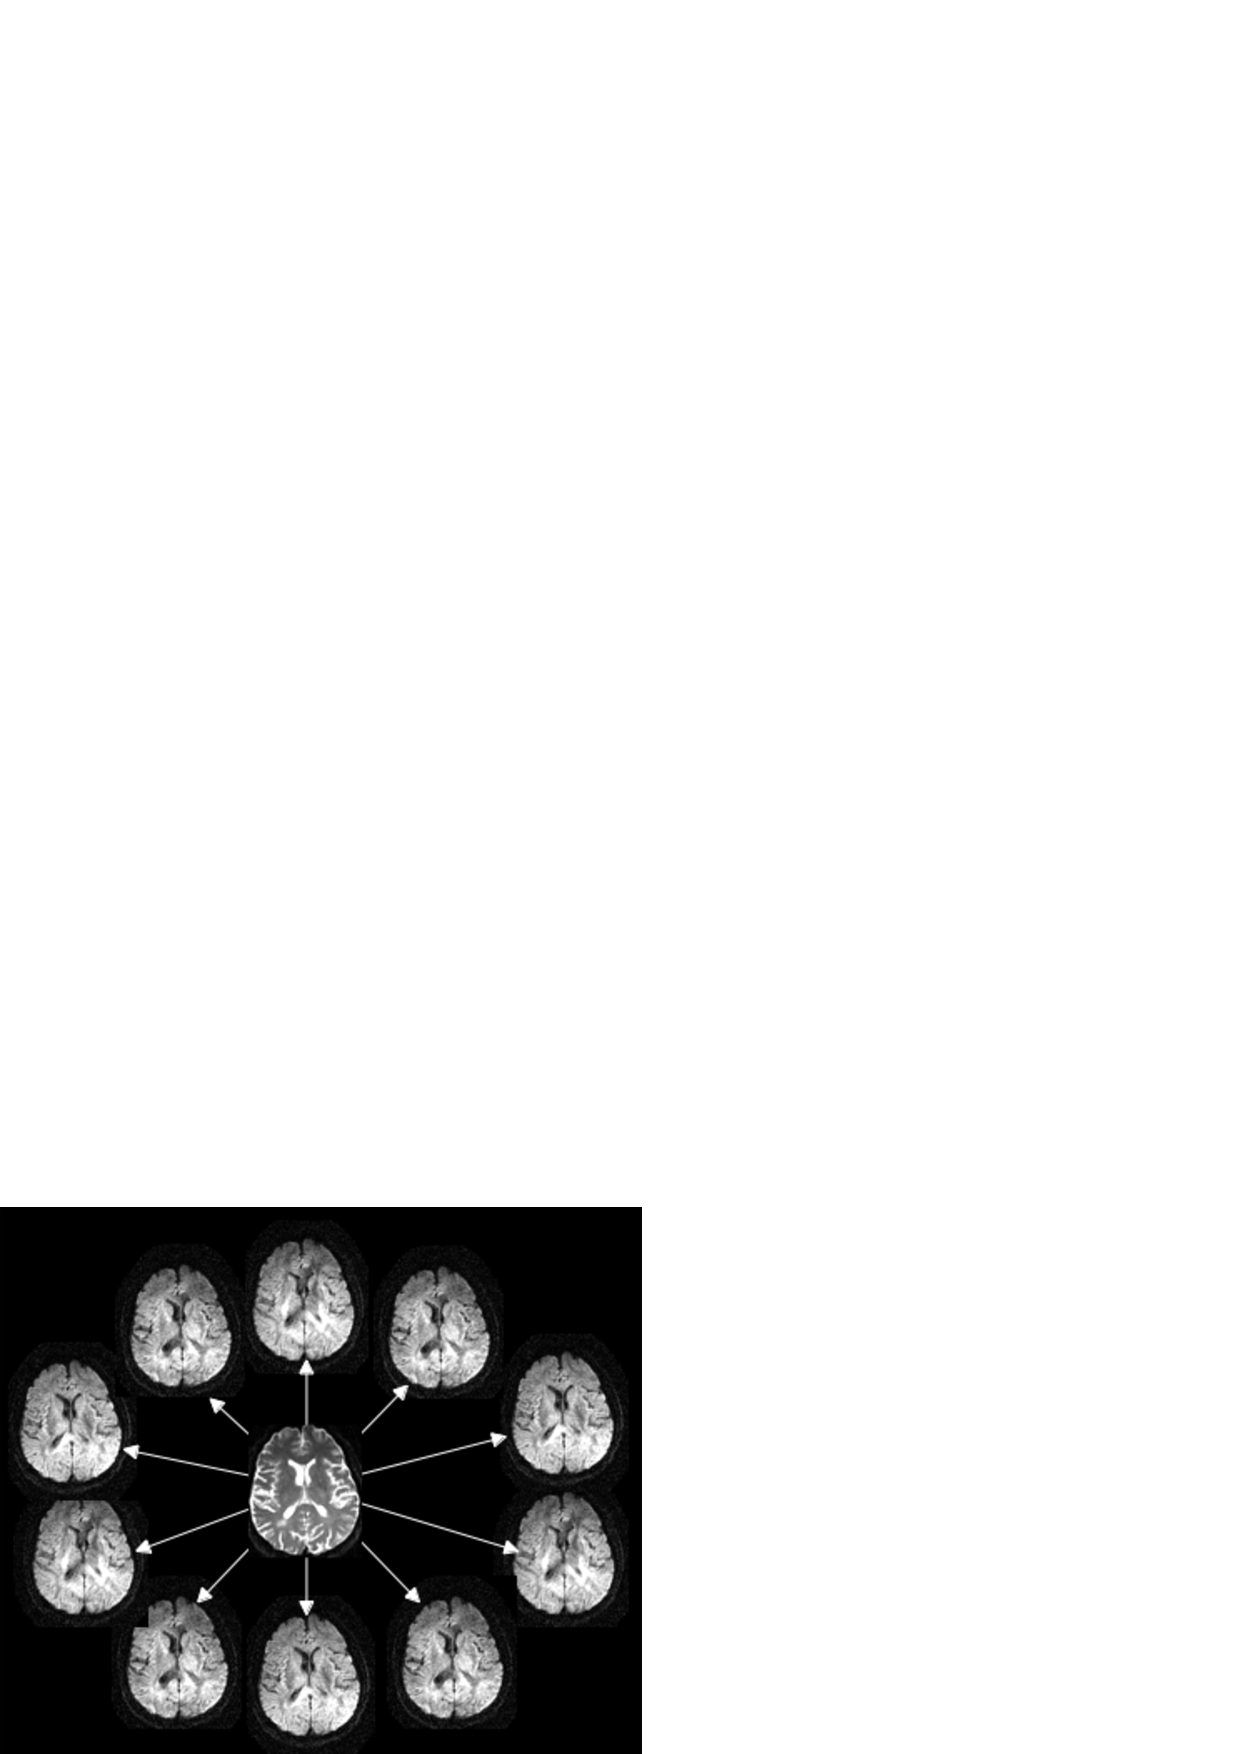
\includegraphics[width=0.5\textwidth]{Images/gradients.pdf}
    \caption{\label{fig:gradients}Les différentes images pondérées en diffusion (images périphériques) 
    et une image pondérée en $T_2$ (image centrale) acquises par une séquence de diffusion.}
\end{figure}

Le terme $\mathbf{g_i^T}\mathbf{D}\mathbf{g_i}$ est un scalaire représentant le Coefficient de Diffusion Apparent ($CDA_i$),
c'est-à-dire la mesure de la diffusion suivant la direction spatiale $\mathbf{g_i}$.
L'écriture de l'équation \eqref{eq:stejskal1965_gauss} peut être simplifiée en notant le signal IRM 
avec gradient de diffusion $S_i$ au lieu de $S(\mathbf{g_i}, b)$.
\begin{equation}
    S_i = S_0 \exp\left( -b \mathbf{g_i^T}\mathbf{D}\mathbf{g_i}\right)
    \label{eq:stejskal1965_simple}
\end{equation}


\section{Tenseur de diffusion}
Dans cette section, nous allons aborder les notions mathématiques fondamentales utilisées pour ce travail de thèse.
Après avoir fait un rappel sur la notion de modèle du tenseur d'ordre 2,
nous verrons comment extraire des indices scalaires représentant certaines informations de la diffusion.
Puis nous verrons la méthode classique d'estimation des tenseurs de diffusion à partir des images pondérées en diffusion.
Enfin, dans un dernier paragraphe, nous présenterons la notion de distance entre deux tenseurs de diffusion ainsi que 
les différentes distances applicables pour des tenseurs d'ordre 2.
% Dans cette section, nous allons aborder les notions mathématiques fondamentales pour comprendre le travail effectué au cours de cette thèse.
% Nous commencerons par faire le point sur la notion de modèle d'ordre 2 
% puis nous verrons comment nous pouvons extraire des indices scalaires représentant certaines informations de la diffusion
% et enfin nous verrons la méthode classique d'estimation des tenseurs de diffusion à partir des images pondérées 
% en diffusion.
% Dans un dernier paragraphe, nous présenterons les différentes distances applicables pour des tenseurs d'ordre 2.\\

Introduit par l'équation \eqref{eq:stejskal1965_gauss}, le tenseur de diffusion $\mathbf{D}$ est un outils mathématique 
qui permet de représenter un objet multi-linéaire, en l'occurence la diffusion de l'eau.
Mathématiquement, un tenseur de diffusion d'ordre $l$ est représenté par un tableau à $p$ dimensions, \underline{défini positif et symétrique}.
Dans la littérature, le modèle d'ordre $l=2$ avec une dimension $p=3$ est le plus fréquemment utilisé~\cite{Basser1994}.
Pour être plus précis, dans le cas de la diffusion, il correspond à la matrice de covariance du déplacement des molécules d'eau.


\subsection{Modèle d'ordre 2}
Le modèle d'ordre 2 du tenseur de diffusion modélise les Coefficients de Diffusion Apparent $CDA_{i=1\dots I}$ sous une forme quadratique \eqref{eq:forme_quatradique}
pour chaque $\mathbf{g_i} = \left[g_{x,i},\ g_{y,i},\ g_{z,i}\right]_{i=1\dots I}$ des $I$ directions de gradients comme vecteurs unitaires.
Cela revient à décomposer le tenseur $\mathbf{D}$ sur une base de polynômes homogènes avec des termes ayant le même degré.
\begin{align}
    CDA_i &= \mathbf{g_i}^T\mathbf{D}\mathbf{g_i} \nonumber \\ 
      &=\sum_{i=1}^{3} \sum_{j=1}^{3} D_{ij}g_ig_j
    \label{eq:forme_quatradique}
\end{align}

Le tenseur de diffusion prend la forme d'une matrice définie positive de dimension 3 avec $3^2$ éléments :
\begin{equation}
    \mathbf{D} = \left[\begin{array}{ccc}
	D_{xx} & D_{xy} & D_{xz}\\
	* & D_{yy} & D_{yz}\\
	* & * & D_{zz}
	\end{array}\right] 
    \label{eq:tenseur_mat}
\end{equation}
\noindent avec $*$ représentant les éléments symétriques de la matrice.

La matrice de diffusion est définie dans le repère physique du scanner IRM $\{\mathbf{x,y,z}\}$.
Il semble plus intéressant de représenter cette diffusion dans un référentiel propre au patient.
Pour cela, une décomposition spectrale \eqref{eq:decomp_spec} permet d'exprimer la matrice $\mathbf{D}$
sur une base de vecteurs propres $\{\mathbf{e_1,e_2,e_3}\}$.
\begin{equation}
    \mathbf{D}\mathbf{e_i} = \lambda_i \mathbf{e_i}
    \label{eq:decomp_spec}
\end{equation}
La transformée de la matrice $\mathbf{D}$ sur cette base est une matrice diagonale 
avec les valeurs propres associées $\{\lambda_1,\lambda_2,\lambda_3\}$ comme éléments diagonaux.
Vu que le tenseur de diffusion est une matrice définie positive à éléments réels et symétrique, 
ses valeurs propres sont positives et réelles.
Ainsi exprimé, le tenseur est représenté dans le repère de la matrice diagonale $\{\mathbf{e_1,e_2,e_3}\}$.

Les vecteurs propres représentent les trois axes de la diffusion avec le vecteur propre $\mathbf{e_1}$
correspondant à la direction principale de la diffusion.
Les valeurs propres sont ordonnées de manière décroissante : $\lambda_1 \geq \lambda_2 \geq \lambda_3$ 
et correspondent à la diffusivité le long de chaque axe respectif.
De cette manière, il est possible de modéliser le phénomène de la diffusion par une ellipsoïde,
comme le schématise la \figref{fig:tenseur}.

\begin{figure}[ht]
    \centering
    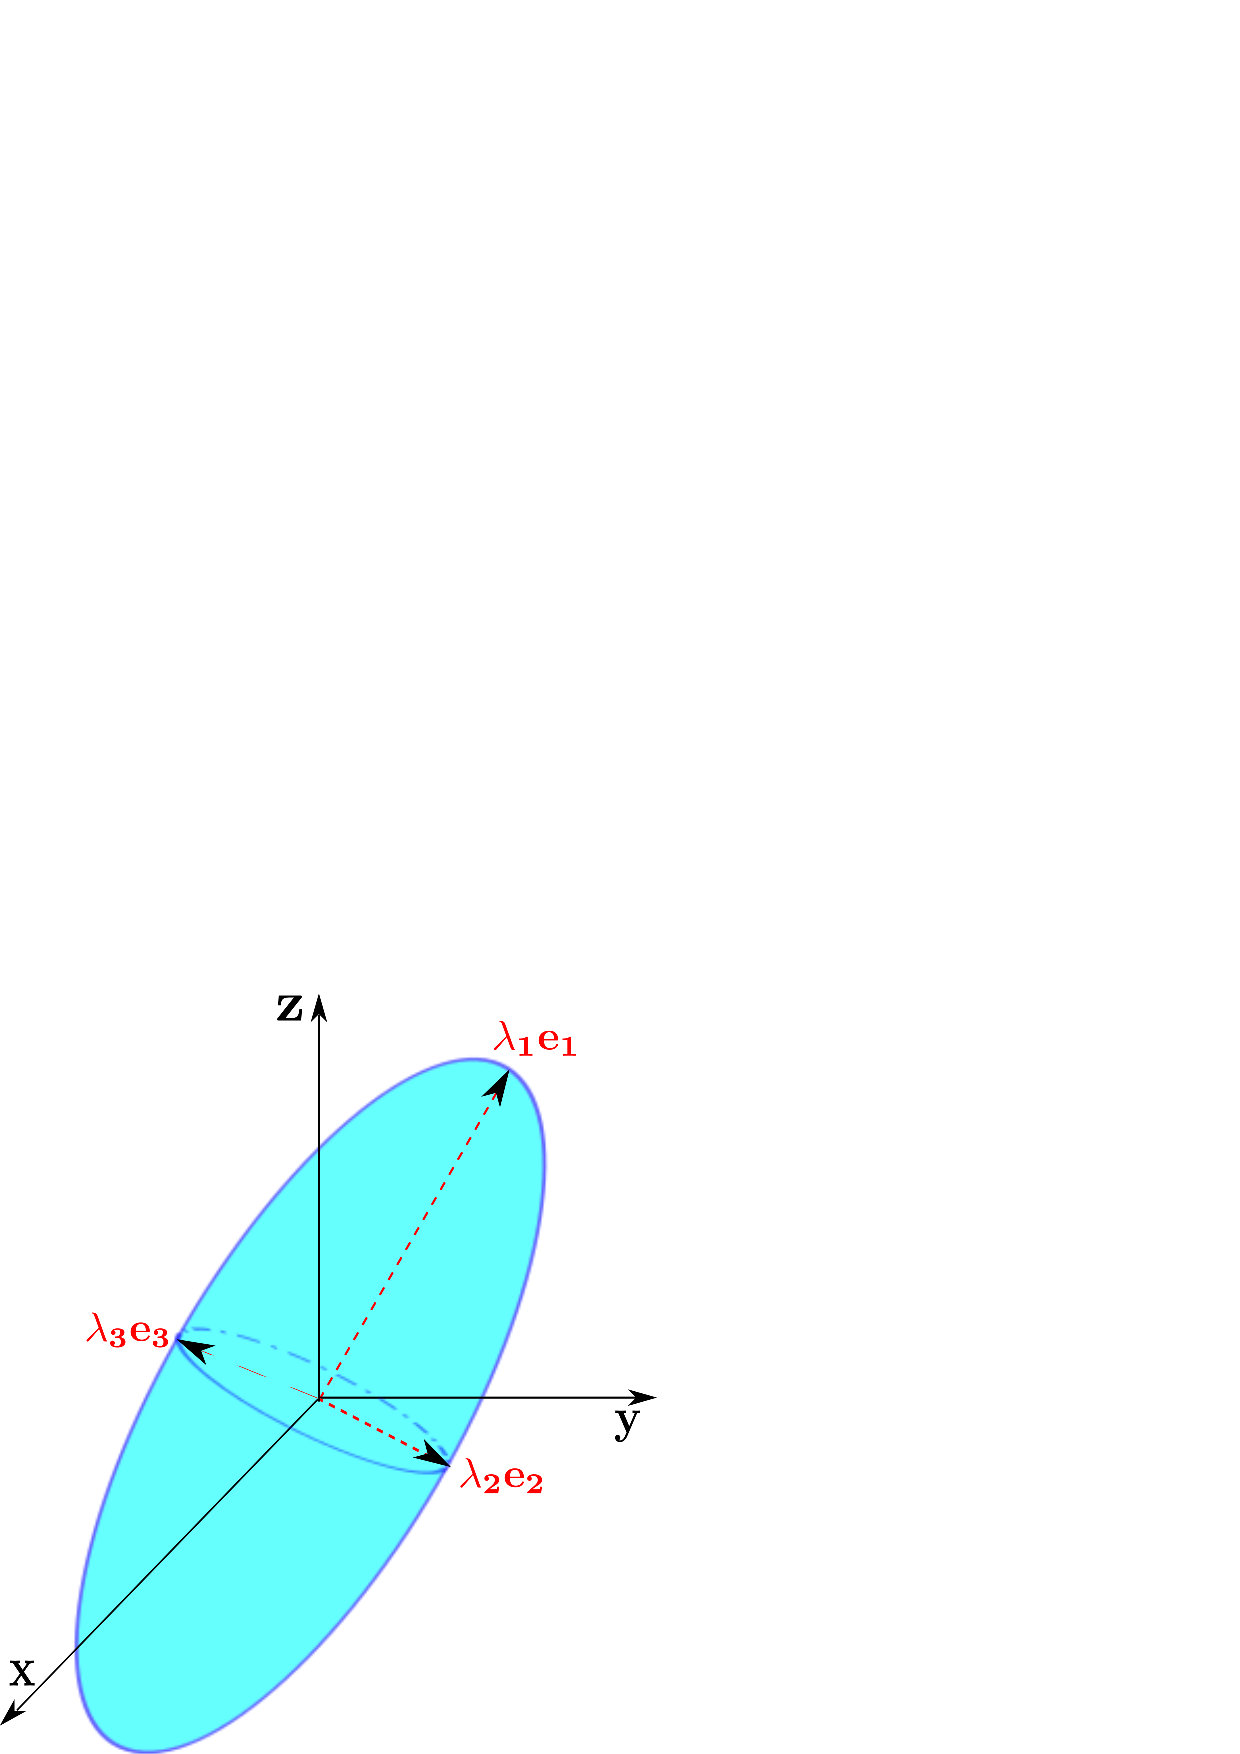
\includegraphics[width=0.4\textwidth]{Images/tensor.pdf}
    \caption{\label{fig:tenseur}Représentation d'un tenseur de diffusion sous la forme d'une ellipsoïde 
    avec le référentiel physique du scanner IRM $\{\mathbf{x,y,z}\}$
    et le référentiel de la matrice diagonale $\{\mathbf{e_1,e_2,e_3}\}$.}
\end{figure}

L'ellipsoïde est définie par trois axes $\{\mathbf{e_1,e_2,e_3}\}$ et trois scalaires $\{\lambda_1,\lambda_2,\lambda_3\}$
qui nous renseigner sur le type de diffusion modélisée.
Il est possible de classer les tenseurs suivant leur forme géométrique définie par les trois scalaires :
\begin{itemize}
    \item les tenseurs à forme sphérique : $\lambda_1 \simeq \lambda_2 \simeq \lambda_3$.
	  Ils dénotent d'une diffusion isotrope: les molécules d'eau se déplacent dans les trois directions de l'espace sans aucune contrainte.
    \item les tenseurs à forme planaire : $\lambda_1 \simeq \lambda_2 \gg \lambda_3$.
	  Dans ce cas, la diffusion est anisotrope car les particules rencontrent une contrainte suivant une des directions.
    \item les tenseurs à forme linéaire : $\lambda_1 \gg \lambda_2 \simeq \lambda_3$.
	  Ces tenseurs sont restreints dans deux des directions de l'espace: ils ont une diffusion dite anisotrope.
\end{itemize}
Pour compléter ce classement sur la diffusion, il est possible, à partir des trois valeurs propres,
de calculer différents paramètres de diffusion que nous appellons \og indices scalaires \fg.
Comme nous le verrons dans le chapitre suivant (\chapref{Chapter2}), l'étude de la forme géométrique d'un tenseur 
peut nous renseigner sur les mécanismes d'une pathologie affectant l'organisation des microstructures cérébrales.


\subsection{Indices scalaires}
Les indices scalaires représentent chacun une unique information sur la diffusion.
Seuls, ils caractérisent partiellement la diffusion, mais vu qu'ils apportent des informations complémentaires,
ils peuvent être combinés et ainsi caractériser totalement la diffusion.\\

Quatre indices scalaires sont les plus souvent utilisés :
\begin{itemize}
    \item La \fa (FA) renseigne sur l'anisotropie de la diffusion. 
    Une valeur de FA grande ($FA=1$) signifie que la diffusion est anisotrope (elle suit un direction privilégiée).
    À l'inverse, une valeur faible de FA correspond à une diffusion isotrope.
    \begin{equation}
        FA = \sqrt{\frac{1}{2}\frac{(\lambda_1 -\lambda_2)^2 + (\lambda_1 -\lambda_3)^2 + (\lambda_3 -\lambda_2)^2 }{\lambda_1^2 + \lambda_2^2 + \lambda_3^2}}
        \label{eq:fa}
    \end{equation}
    \item La \md (DM) indique si la diffusion globale, c'est-à-dire dans les trois directions, est restreinte (DM petite) ou sans contrainte (DM élévée).
    \begin{equation}
        DM = \frac{\lambda_1 + \lambda_2 + \lambda_3}{3}
        \label{eq:md}
    \end{equation}
    \item La \dr (DR) caractérise la diffusion suivant les deux axes secondaires :
    \begin{equation}
	DR = \frac{\lambda_2 + \lambda_3}{2}
        \label{eq:dr}
    \end{equation}
    \item La \da (DA) correspond à la valeur propre associée à la direction principale :
    \begin{equation}
	DA = \lambda_1
        \label{eq:da}
    \end{equation}
\end{itemize}

De nombreux autres indices scalaires peuvent être calculés tels que le mode ou encore l'anisotropie relative.
Cependant, durant la thèse, seuls ces quatre indices scalaires sont utilisés.
La \figref{fig:scalaires} montre trois coupes différentes pour chacun des quatre indices scalaires pour un même sujet.


\subsection{Estimation par les moindres carrés}
L'image contenant en chaque voxel un tenseur de diffusion (modèle d'ordre 2) n'est pas obtenue directement lors d'une séquence d'IRM de diffusion.
Nous avons vu que nous acquierons une série d'images pondérées en diffusion suivant différentes directions.
À partir de cette séquence d'images acquises, il est possible d'estimer les tenseurs de diffusion en chaque voxel du volume 3D.
Nous parlons alors d'\itd (ITD).

La méthode, la plus communément utilisée, est l'estimation au sens des moindres carrés (LS pour \textit{Least Squares}).
Elle permet d'estimer, voxel par voxel, le tenseur d'ordre 2 correspondant.
Elle consiste à résoudre un système linéaire en minimisant l'erreur quadratique entre les données et les estimées.
Pour construire le système linéaire, nous repartons de l'équation \eqref{eq:stejskal1965_simple} 
et nous linéarisons son expression en passant au logarithme.
Nous rappelons qu'il y a $\mathbf{g_{i=1\dots I}}$ gradients de diffusion.
\begin{align}
    \ln \left(\frac{S_i}{S_0}\right) &= -b \mathbf{g_i^T}\mathbf{D}\mathbf{g_i} \nonumber \\
    \ln \left(S_i\right) &= \ln \left(S_0\right) - b \mathbf{g_i^T}\mathbf{D}\mathbf{g_i} \nonumber
\end{align}

La dernière équation peut se réécrire sous la forme matricielle.
Pour un soucis de place, nous avons mis la négation sur les 6 termes du tenseur de diffusion.
\begin{equation}
    \left[\begin{array}{c}
              \ln \left(S_1\right) \\
              \vdots \\
              \ln \left(S_i\right) \\
              \vdots \\
              \ln \left(S_I\right) \\
          \end{array}\right]  = \left[\begin{array}{ccccccc}
				      1 & bg_{1,x}^2 & 2bg_{1,x}g_{1,y} & 2bg_{1,x}g_{1,z} & bg_{1,y}^2 & 2bg_{1,y}g_{1,z} & bg_{1,z}^2\\
				      \vdots & \vdots & \vdots & \vdots & \vdots & \vdots & \vdots \\
                                     1 & b g_{i,x}^2 & 2bg_{i,x}g_{i,y} & 2bg_{i,x}g_{i,z} & bg_{i,y}^2 & 2bg_{i,y}g_{i,z} & bg_{i,z}^2 \\
                                     \vdots & \vdots & \vdots & \vdots & \vdots & \vdots & \vdots \\
                                     1 & b g_{I,x}^2 & 2bg_{I,x}g_{I,y} & 2bg_{I,x}g_{I,z} & bg_{I,y}^2 & 2bg_{I,y}g_{I,z} & bg_{I,z}^2 
                                 \end{array}\right] \left[\begin{array}{c}
							  \ln\left(S_0\right) \\
							  -D_{xx}\\
							  -D_{xy}\\
							  -D_{xz}\\
							  -D_{yy}\\
							  -D_{yz}\\
							  -D_{zz}\\
						      \end{array}\right]	\nonumber
\end{equation}

Nous nous retrouvons face à un système d'équations à 7 inconnues
sous la forme $\mathbf{A} = \mathbf{B}\mathbf{x}$ avec $\mathbf{x}$ le vecteur d'inconnues à estimer.
Pour obtenir une solution à ce système, il est nécessaire d'avoir au minimum $I=7$ équations : 
il faut donc acquérir 7 images pondérées en diffusion avec 7 gradients de diffusion différents. 
La méthode des moindres carrés cherche un solution qui minimise l'erreur quadratique dûe à l'estimation
$\mathbf{\hat{x}} = \arg\min_{\mathbf{x} \in \mathbb{R}^{7}}{\|\mathbf{A} - \mathbf{B}\mathbf{x} \|^{2}}$.
Cela se traduit par une pseudo-inversion matricielle \eqref{eq:pseudoinverse} :
\begin{equation}
    \mathbf{\hat{x}} = (\mathbf{B}^{t}\mathbf{B})^{-1}\mathbf{B}^{t}\mathbf{A}
    \label{eq:pseudoinverse}
\end{equation}

L'\algoref{algo:estimation_tenseur} de cette estimation détaille le pseudo-code implémenté.
\begin{center}
    \begin{minipage}[c]{0.95\textwidth}
	\begin{algorithm}[H]
	    \vspace*{0.5em}
	    \Data{
		$log(S_i) = z_i^t\theta + \epsilon_i$
		$\text{avec  } z_i^t = (1, -b(g_{i,x}^2, 2g_{i,x}g_{i,y}, 2g_{i,x}g_{i,z}, g_{i,y}^2, 2g_{i,y}g_{i,z}, g_{i,z}^2))$
		$\text{et  }\theta = (log(S_0), D_{xx}, D_{xy}, D_{xz}, D_{yy}, D_{yz}, D_{zz})$}\vspace*{1em}
	    \Res{Estimation des 7 paramètres de $\theta$ : $\hat{\theta} = (log(S_0), D_{xx}, D_{xy}, D_{xz}, D_{yy}, D_{yz}, D_{zz})$}\vspace*{1em}
	    \Sortie{$\hat{\theta} = ( \sum_{i=1}^{I} z_i z_i^t )^{-1} \sum_{i=1}^{I} z_i\ log(S_i)$}\vspace*{0.5em}
	    \caption{\label{algo:estimation_tenseur}Estimation du tenseur de diffusion par les moindres carrés}
	\end{algorithm}
    \end{minipage}
\end{center}

Contrairement aux thèses précédentes \cite{Boisgontier_PhD, Grigis_PhD}, nous estimons également l'image $S_0$ pondérée en $T_2$.
De cette manière, lorsque nous rencontrons le cas de multiples images $S_0$, 
la question de savoir s'il faut prendre, pour l'estimation du tenseur, la première de ces images
ou bien faire leur moyenne ne se pose pas.

Cependant, cette estimation (au sens des moindres carrés) présente plusieurs limites.
Premièrement, cette méthode est le meilleur estimateur au sens du maximum de vraisemblance pour un bruit additif gaussien.
Or le bruit de l'acquisition d'un IRM est considéré ricien.
Par conséquent, nous formulons de fortes hypothèses erronées de gaussianité sur les observations en utilisant la méthode des moindres carrés.
Deuxièmement, cette méthode ne garantit pas la positivité des tenseurs.
Différentes solutions à ce problème sont proposées. 
Par exemple, une solution directe et simple en post-estimation consiste à mettre les valeurs propres négatives à 0 
et à reconstruire les tenseurs. 
Ou encore il existe des méthodes d'estimation \cite{Barmpoutis2010} qui prennent en compte la positivité des tenseurs 
mais qui engendrent des calculs de résolution plus complexes.


\subsection{Distances entre deux tenseurs d'ordre 2}
La notion de distance est importante pour la compréhension des travaux de cette thèse.
En effet, le but principal de la compraison de groupes est de regarder 
si la distance entre deux populations de tenseurs de diffusion est statistiquement significative.
Les explications à propos de la compraison de groupe en \itd sont abordées au \chapref{Chapter3}
et un état de l'art sur l'influence du choix de la distance pour mener une comparaison de groupe en ITD est disponible au \chapref{Chapter5}.
Dans ce paragraphe, seules les notions mathématiques relatives aux différentes distances applicables à des tenseurs de diffusion sont présentées.\\

De manière générale, le distance peut être formalisée de la manière suivante :
\begin{adjustwidth}{2cm}{}
    Soit $\mathbb{M}$ une variété et $d:\mathbb{M} \times \mathbb{M} \rightarrow \mathbb{R}^+$ la fonction distance associée à cette variété
    qui vérifie les propriétés suivantes :
    \begin{itemize}
        \item symétrie : $\forall (a,b) \in \mathbb{M}^2, d(a,b)=d(b,a)$
        \item séparation : $\forall (a,b) \in \mathbb{M}^2, d(a,b)=0 \Leftrightarrow a=b$
        \item inégalité triangulaire : $\forall (a,b,c) \in \mathbb{M}^3, d(a,c)\leq d(a,b) + d(b,c)$
    \end{itemize}
    Cette variété est alors un \og espace métrique \fg auquel est rattachée une métrique définissant la distance.
    Suivant la variété, la fonction distance prend une expression mathématique différente.
    En effet, elle mesure la longueur entre deux points appartenant à cette variété en préservant la topologie de l'espace.\\
\end{adjustwidth}

Le tenseur de diffusion d'ordre 2 est une matrice de dimension 3, symétrique et définie positive 
qui peut être associée à trois variétés ayant des topologies différentes :
\begin{itemize}
    \item le domaine Euclidien : $\mathbb{M} \subset \mathbb{R}$,
    \item le domaine Riemannien : $\mathbb{M} \subset Sym^+(3)$,
    \item le domaine Log-Euclidien : $\mathbb{M} \subset Sym(3)$.\\
\end{itemize}

Le domaine Euclidien est un espace vectoriel muni d'un produit scalaire (entre deux matrices)
auquel est associé la norme de Frobenius $\|\mathbf{D}\|=\sqrt{tr(\mathbf{D}^t\mathbf{D})}$.
La distance euclidienne est la norme de Frobenius appliquée à la différence entre deux points du domaine.
\begin{align}
    d_{Euclidien}(\mathbf{D_1}, \mathbf{D_2}) &= \|\mathbf{D_1}-\mathbf{D_2} \| \nonumber \\
    &= \sqrt{tr((\mathbf{D_1}-\mathbf{D_2})^t(\mathbf{D_1}-\mathbf{D_2}))}
\end{align}
Cependant, même si cette distance entre deux réels permet d'obtenir un réel,
lorsqu'elle est appliquée à deux matrices symétriques définies positives, 
elle n'assure pas la positivité du résultat et seule la symétrie est conservée.\\

Ce problème est résolu lorsque la distance Riemannienne \cite{Pennec2006, Fletcher2007} est utilisée.
L'espace Riemannien est un espace courbé, représenté sur la \figref{fig:sphere} par une sphère.
La distance entre deux points de cet espace est un chemin géodésique qui respecte la topologie de l'espace (courbure).
\begin{equation}
    d_{Riemannien}(\mathbf{D_1}, \mathbf{D_2}) = \sqrt{\frac{1}{2} tr\left(\log \left(\mathbf{D_1}^{-\frac{1}{2}}\mathbf{D_2}\mathbf{D_1}^{-\frac{1}{2}} \right)^2 \right)}
\end{equation}


Cependant, d'un point de vue implémentation, cette distance demande des opérations complexes qui peuvent se révéler consommatrices en temps de calcul.
Pour éviter ce désavantage, une nouvelle distance a été définie : la distance Log-Euclidienne \cite{Arsigny2006}.
Elle prend la forme d'une application projetant le tenseur de l'espace $Sym^+(3)$ sur un plan tangent Euclidien (\figref{fig:log_sphere}).
À partir de là, les métriques du domaine Euclidien peuvent être appliquées sur le tenseur projeté.
\begin{align}
    d_{Log-Euclidien}(\mathbf{D_1}, \mathbf{D_2}) &= \|\log \left(\mathbf{D_1}\right)- \log \left(\mathbf{D_2}\right) \|
\end{align}



\begin{figure}[ht]
    \begin{minipage}[c]{0.4\textwidth}
	    \centering
	    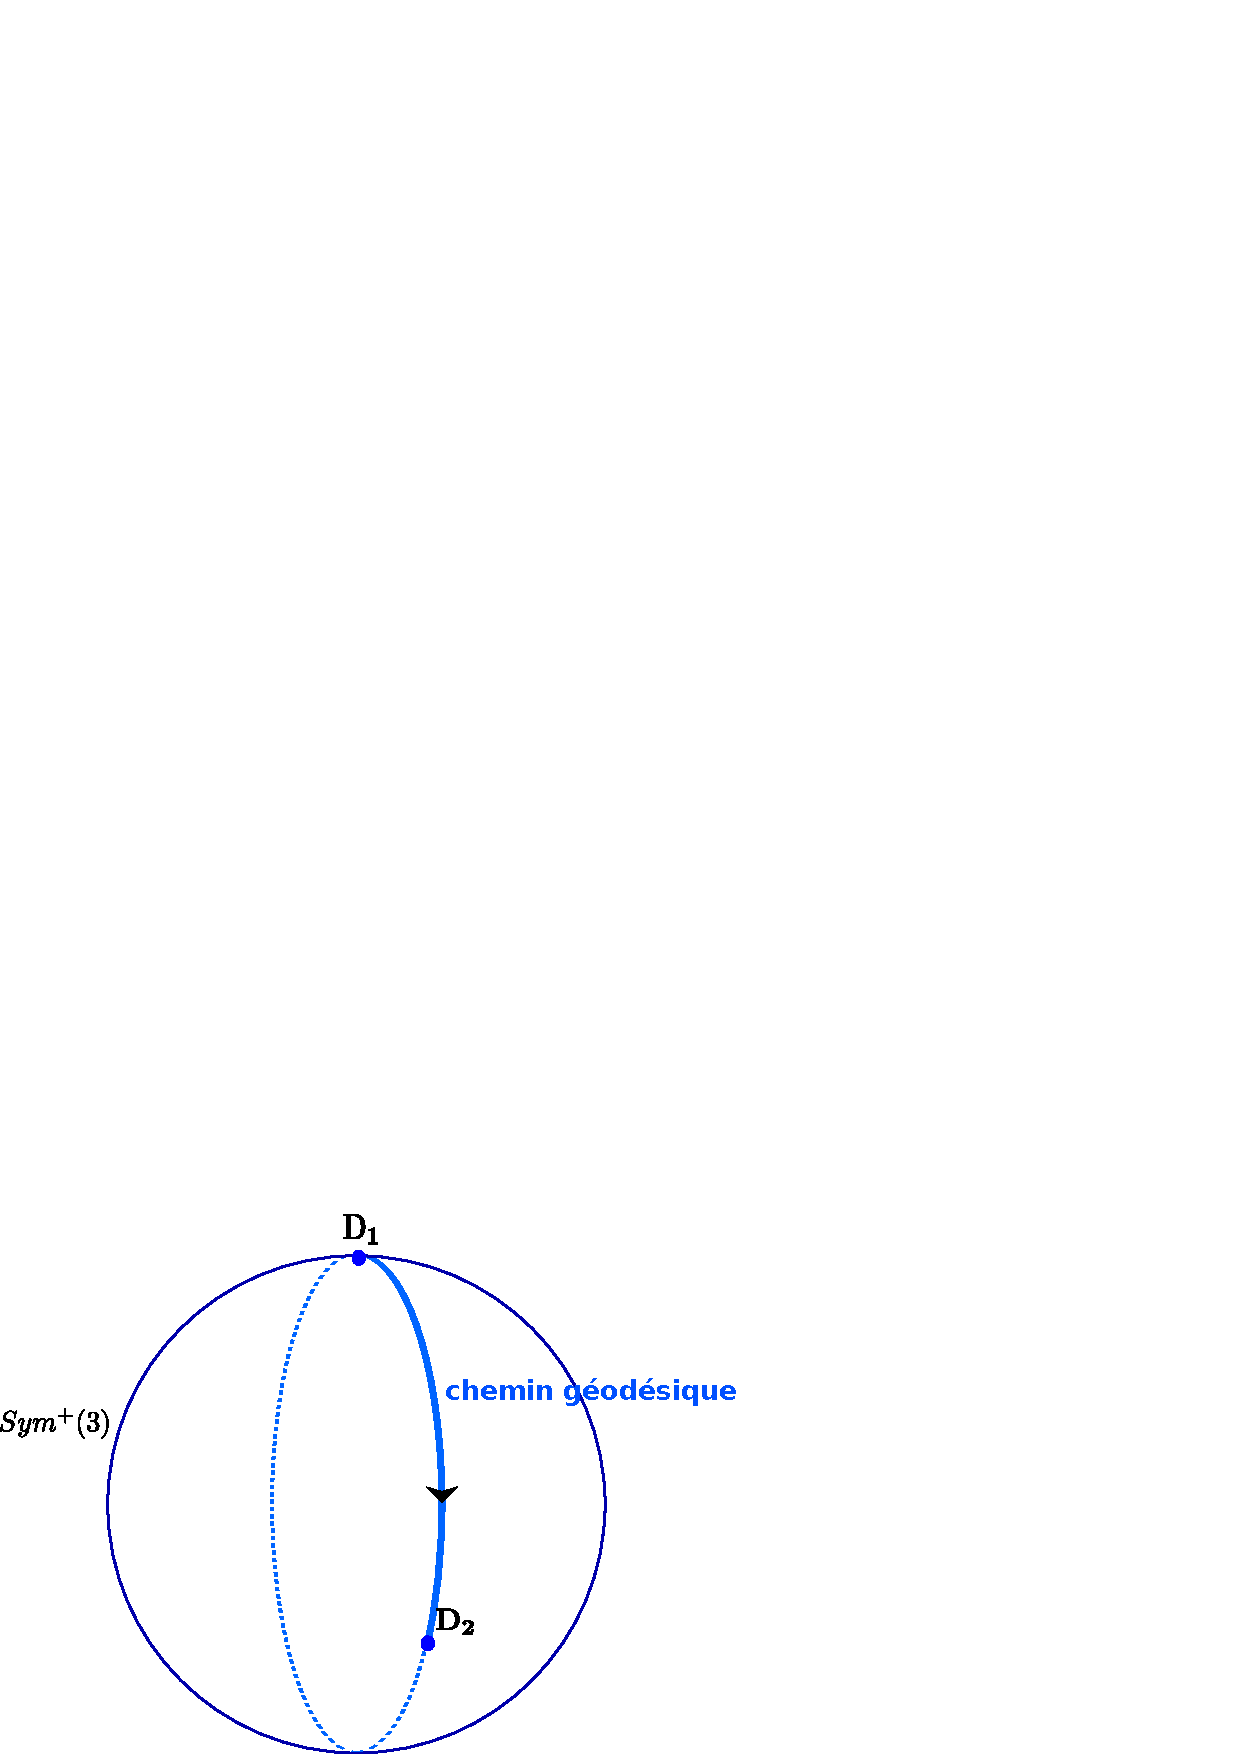
\includegraphics[width=0.85\textwidth]{Images/sphere.pdf}
	    \caption{\label{fig:sphere} Illustration de l'espace Riemannien sous forme de sphère.}
    \end{minipage}\hfill
    \begin{minipage}[c]{0.5\textwidth}
	    \centering
	    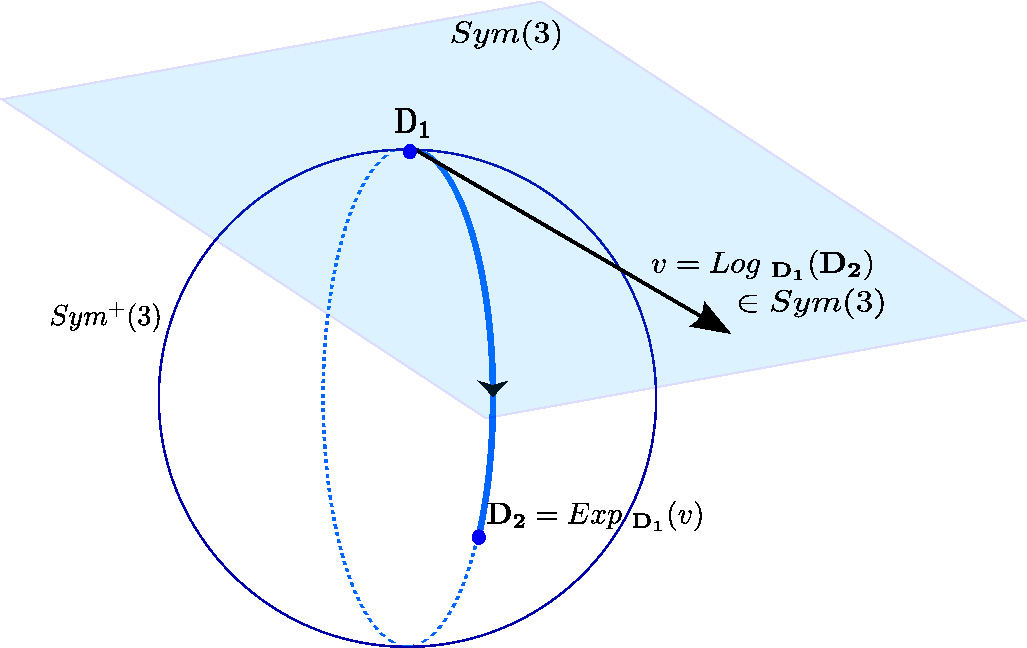
\includegraphics[width=1\textwidth]{Images/log_exp_map_sphere.pdf}
	    \caption{\label{fig:log_sphere} Illustration de l'espace Riemannien avec un plan tangent.}
    \end{minipage}
\end{figure}


\begin{figure}[ht]
    \centering
    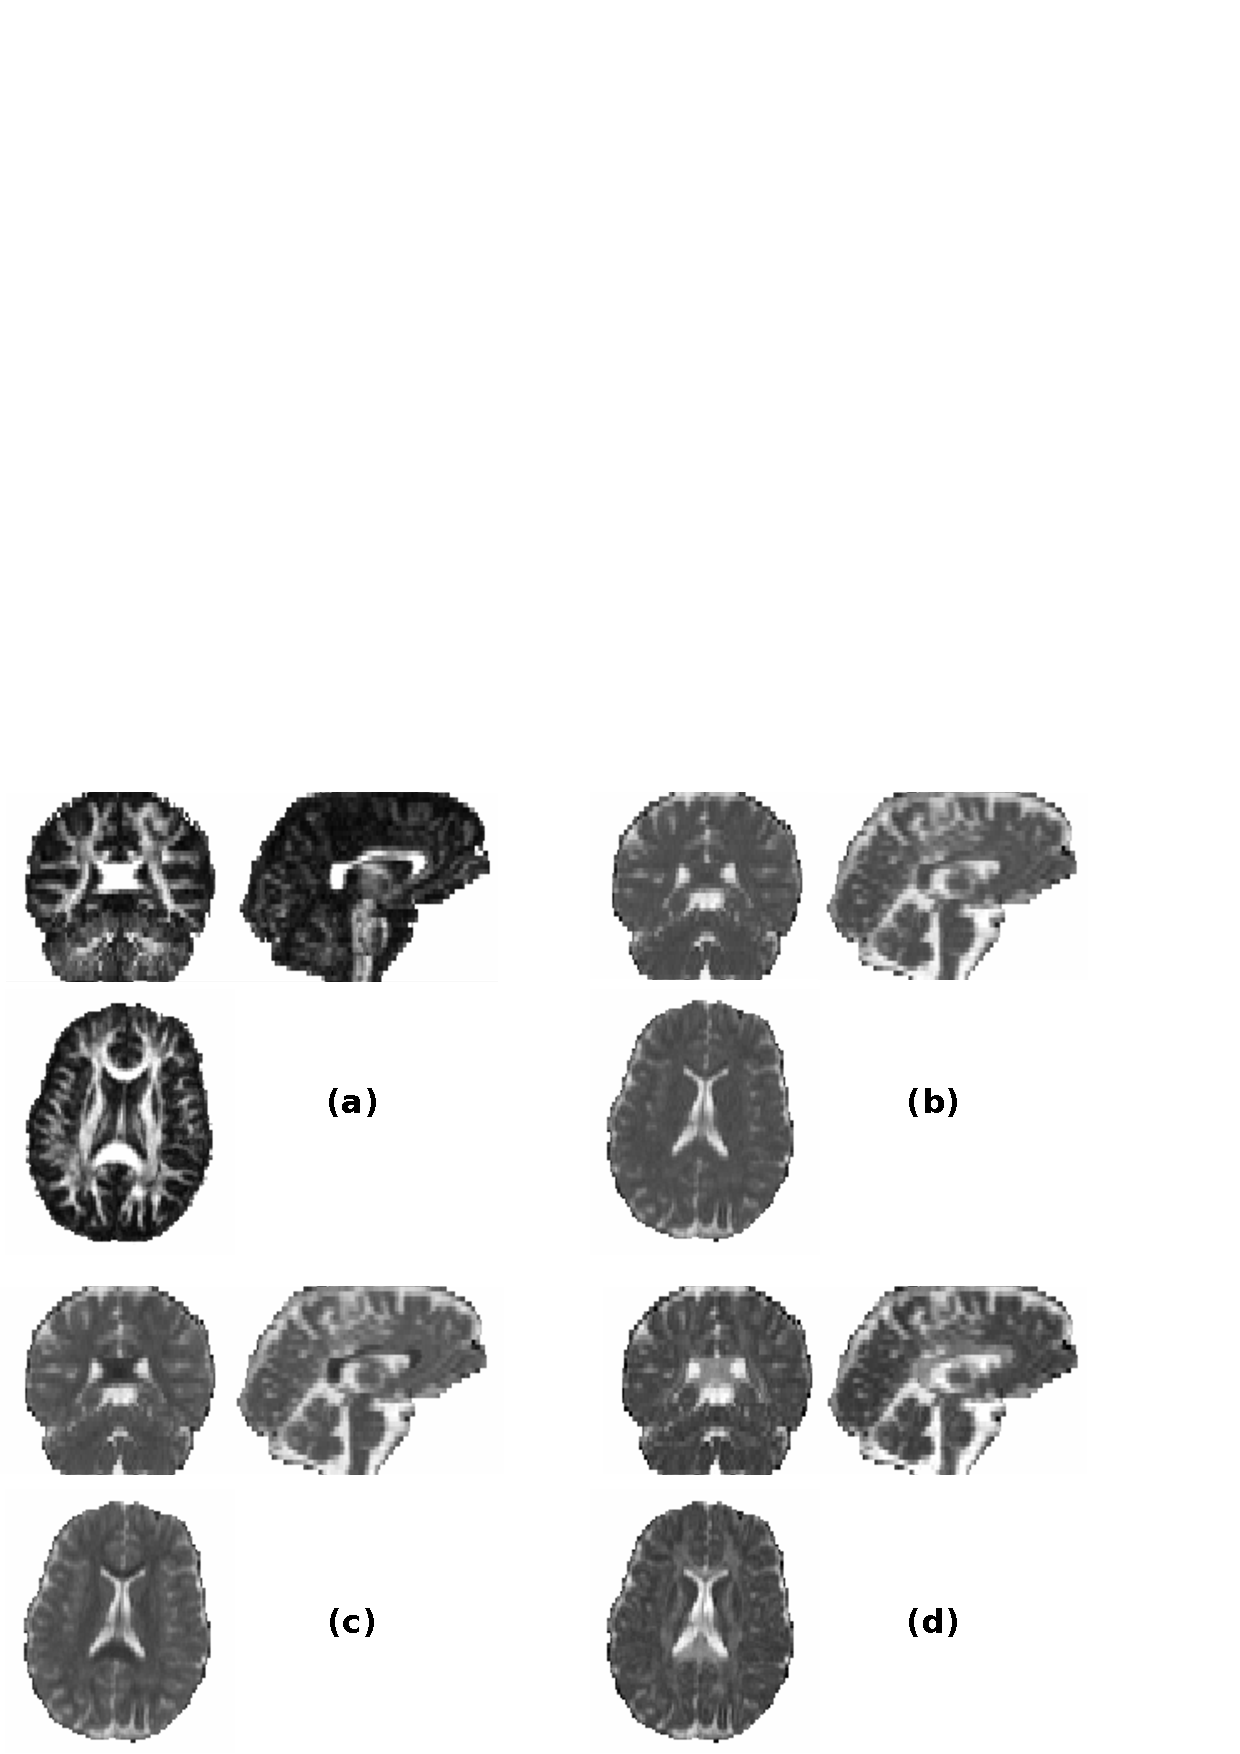
\includegraphics[width=1\textwidth]{Images/scalaires.pdf}
    \caption{\label{fig:scalaires}Images des indices scalaires pour un sujet : \textbf{(a)} FA, \textbf{(b)} DM, \textbf{(c)} DR, \textbf{(d)} DA.}
\end{figure}

